\setcounter{section}{4} % This causes the next section to be Appendix B


\section*{Examples IV. 3D Time-dependent Behavior Examples}
\label{PS4}

This set of example problems is due on November 17, 2025. 

\medskip
\subsection*{4--1. \textbf{Characterization with deflection history} [4 pts].} 
A simply supported beam is made from a material that is well-described by a three-parameter standard linear solid model, i.e., the general creep compliance function $J_c(t)$ is given by
\begin{equation*}
    J_c(t) = J_\infty + (J_0 - J_\infty) \exp\left[-\frac{t}{\tau_c}\right],
\end{equation*}
where $J_\infty$, $J_0$, and $\tau_c$ are all mechanical properties of the material. 

The beam has a length of 4 ft and a second moment of area about the out-of-plane axis of 1 in$^4$. 
It is subjected to a position-time separable load function $q(z,t) = \hat{q}(z) \phi(t)$ where $\phi(t) = -3$ lb/ft $\cdot \mathcal{H}(t)$. 
Say we determine the maximum deflection in the beam at different times to be
\begin{align}
    &u_y \Big|_{\max} = -0.6 \textrm{~in~~at~~}t=30\textrm{~min}\\
    &u_y \Big|_{\max} = -0.75 \textrm{~in~at~~}t=60\textrm{~min}\\
    &u_y \Big|_{\max} = -1.0 \textrm{~in~~at~~}\textrm{~long times}
    \end{align}
From this, calibrate the material properties.

\bigskip
\subsection*{4--2. \textbf{Ramp up the torque} [4 pts].} 
A viscoelastic cylinder $AB$ is fixed on its end $A$ and simply supported on its opposite end at $B$. 
At point $B$, a second, rigid rod is joined to the end such that exerting a force on the rod will induce a counterclockwise torque about the axis of $AB$. 
A point force of magnitude $P_0$ is applied to the rigid rod, causing the front face to turn counterclockwise. 
The point force travels along the rod such that its distance from the bar's neutral axis $a(t)$ is direct in time, i.e., $a(t) = \alpha t$, where $\alpha$ is a constant. 
What is the angular rotation of the end $B$ as a function of time, $\Phi(t)$?

\bigskip
\subsection*{4--3. \textbf{L-shaped beam} [4 pts].}
\begin{wrapfigure}[8]{r}{2in}
\vspace{-1cm}
    \centering
     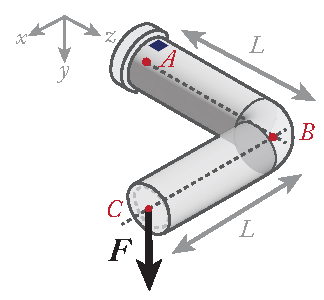
\includegraphics[scale=1]{instr-figures/L-bracket.pdf}
    \caption*{Figure 4.3a.}
    \label{fig:Lbracket}
\end{wrapfigure}
A one-piece polymeric member \textit{ABC} consists of two segments of length $L$ at a right angle from one-another and encastred at $A$, as shown. 
Its neutral axes both lie in the $x-z$ plane when unloaded. 
Assuming the creep compliance in shear to be $\mu_c{t}$ and the creep compliance in axial tension to be $E_c(t)$, determine (a) the deflection at $C$ in terms of the time-varying force $F(t)$ and (b) the stress tensor $\mathbf{\sigma}(t)$ at the square surface element located above $A$.  

\newpage
\subsection*{4--4. \textbf{Fibrous material} [4 pts].}
An elastic material with a fiber phase has the Helmholtz free energy function
\begin{equation*}
\widetilde{\psi}(\bn{F}) = \frac{1}{2}C_{10} (I_1-3) + \frac{1}{4} k (I_a - 1)^2,
\end{equation*}
where $I_1(\bn{C}) = \textrm{tr}(\bn{C})$ and $I_a(\bn{C},\hat{\bm{a}}_0) = \hat{\bm{a}}_0 \cdot \bn{C} \hat{\bm{a}}_0$ for $\bn{C} = \bn{F}^\intercal \bn{F}$.

%\skiponeline
%(a) Show that, given the direction $\hat{\bm{a}}_0$ is fixed by the material, $I_a$ is an invariant of $\bn{C}$.

\medskip
(a) Show that this elastic potential is consistent with the principle of objectivity.

\medskip
(b) Show that the material symmetry group $\mathcal{G}$ is the set of all proper orthogonal tensors $\bn{H}$ with $\bn{H}\hat{\bm{a}}_0 = \hat{\bm{a}}_0$.  

\medskip
(c) Find the first Piola-Kirchhoff and Cauchy stress expressions with an applied deformation gradient tensor of $\bn{F}$.


\bigskip
\bigskip
\subsection*{4--5. \textbf{Gent model of rubber elasticity} [4 pts].}
The Gent model, which incorporates the finite extensibility of polymer chains in a rubber network but includes $I_2$-dependence, has a free-energy function of $$\bar{\Psi} = -\frac{C_{10}}{2} J_m \ln \left(1 - \frac{I_1-3}{J_m} \right) + C_{01}\ln \left(\frac{I_2}{3}\right), $$ where $C_{10}>0$, $C_{01}\geq 0$, and $J_m>0$ are material constants.

\medskip
(a) Show that the Cauchy stress corresponding to the free energy above has the form $$\bm{\sigma} = -p \bn{I} + \frac{C_{10} J_m}{J_m - (I_1-3)}\bn{B} - \frac{2C_{01}}{I_2} \bn{B}^{-1}.$$

\medskip
(b) This material undergoes a simple shear deformation of magnitude $\gamma$. Given that the shear modulus $\mu(\gamma^2) \equiv \beta_1(\gamma^2) - \beta_{-1} (\gamma^2)$ where $\beta_i$ corresponds to the expression for $\bm{\sigma}$ in Q1, show that in the small strain limit that $$\lim\limits_{\gamma \rightarrow 0} \mu(\gamma^2) = C_{10} + \frac{2}{3} C_{01}.$$
